\subsection{Preemptible functions: \textit{libinger}}
\label{sec:libinger}

We now introduce libinger, a library providing a timed function abstraction via the
\texttt{launch()}/\texttt{resume()} interface proposed at the beginning of the
section.  The library provides bindings for the C and Rust systems programming
languages; while its abstraction should work in any language whose runtime supports
stack unwinding (including any language with exceptions), we leave it to future work
to develop bindings for other languages via their respective foreign-function
interfaces.

In designing their centralized preemption thread, the Shinjuku authors conducted a
study comparing the latency of bare-metal interprocessor interrupts (IPIs) against
that of Linux signals.  While their results show that IPIs take an average of only
1993 cycles, compared to 4950 for signals, their sender/receiver breakdown reveals
that between 343 and 2084 of the cycles associated with the latter overhead are
incurred by the sender~\cite{Kaffes:nsdi2019}.  This suggests that a timer-based
design where the client subscribes once to a repeating signal may come within 873
cycles (about 400 ns on a 2-GHz processor) of the preemption latency possible with
bare-metal IPIs.

We base our preemption mechanism on that employed by RT, which uses a POSIX timer to
repeatedly trigger their \texttt{RELEASE\_SIGNAL}, whose handler forwards the
notification to other worker threads by \texttt{kill()}'ing them with a second
signal, \texttt{PREEMPTION\_SIGNAL}~\cite{mollison:rtas2013}.  To avoid the sender
overhead, we need to eliminate the two-phase signaling, ideally by just subscribing
each thread to the same \texttt{RELEASE\_SIGNAL}.  Unfortunately, according to the
Linux Programmer's Manual~\cite{signal-manpage}, ``A process-directed signal may be
delivered to any one of the threads that does not currently have the signal blocked.
If more than one of the threads has the signal unblocked, then the kernel chooses an
arbitrary thread to which to deliver the signal.''  We work around this limitation by
configuring a different POSIX timer with its own signal for each thread that is
currently executing a preemptible function.  All threads use the same handler, but
store their preemption signal in a thread-local variable.  Whenever the handler runs,
it checks whether it was triggered by the current thread's signal.  If not, it masks
the rogue signal and immeditely returns; in this way, the system quickly converges on
delivering each preemption signal only to its corresponding thread.  The current
implementation sets each timer to fire at a fixed scheduling interval in the tens of
microseconds.

\solb{We probably want to select the quantum dynamically based on the requested
timeout; otherwise, cite our ATC paper to justify the fixed quantum.}

Because we want to support resuming preempted functions, we must run each preemptible
function on its own stack.  As such, whenever \texttt{launch()} is called, it creates
a \textbf{checkpoint} continuation using \texttt{getcontext()}, allocates a
fixed-size stack and uses the POSIX \texttt{makecontext()} and \texttt{setcontext()}
functions to switch to it.  It then allocates a preemption signal from a pool of
rarely-used signal numbers if there isn't already one assigned to the thread,
enables a POSIX timer via \texttt{timer\_settime()}, allocates and switches to a
libgotcha libset, and calls the user-provided preemptible function.
Figure~\ref{fig:dispatch} shows a high-level view of a call to \texttt{launch()}, as
well as a call into a shared symbol from within the invoked timed function.

\begin{figure}
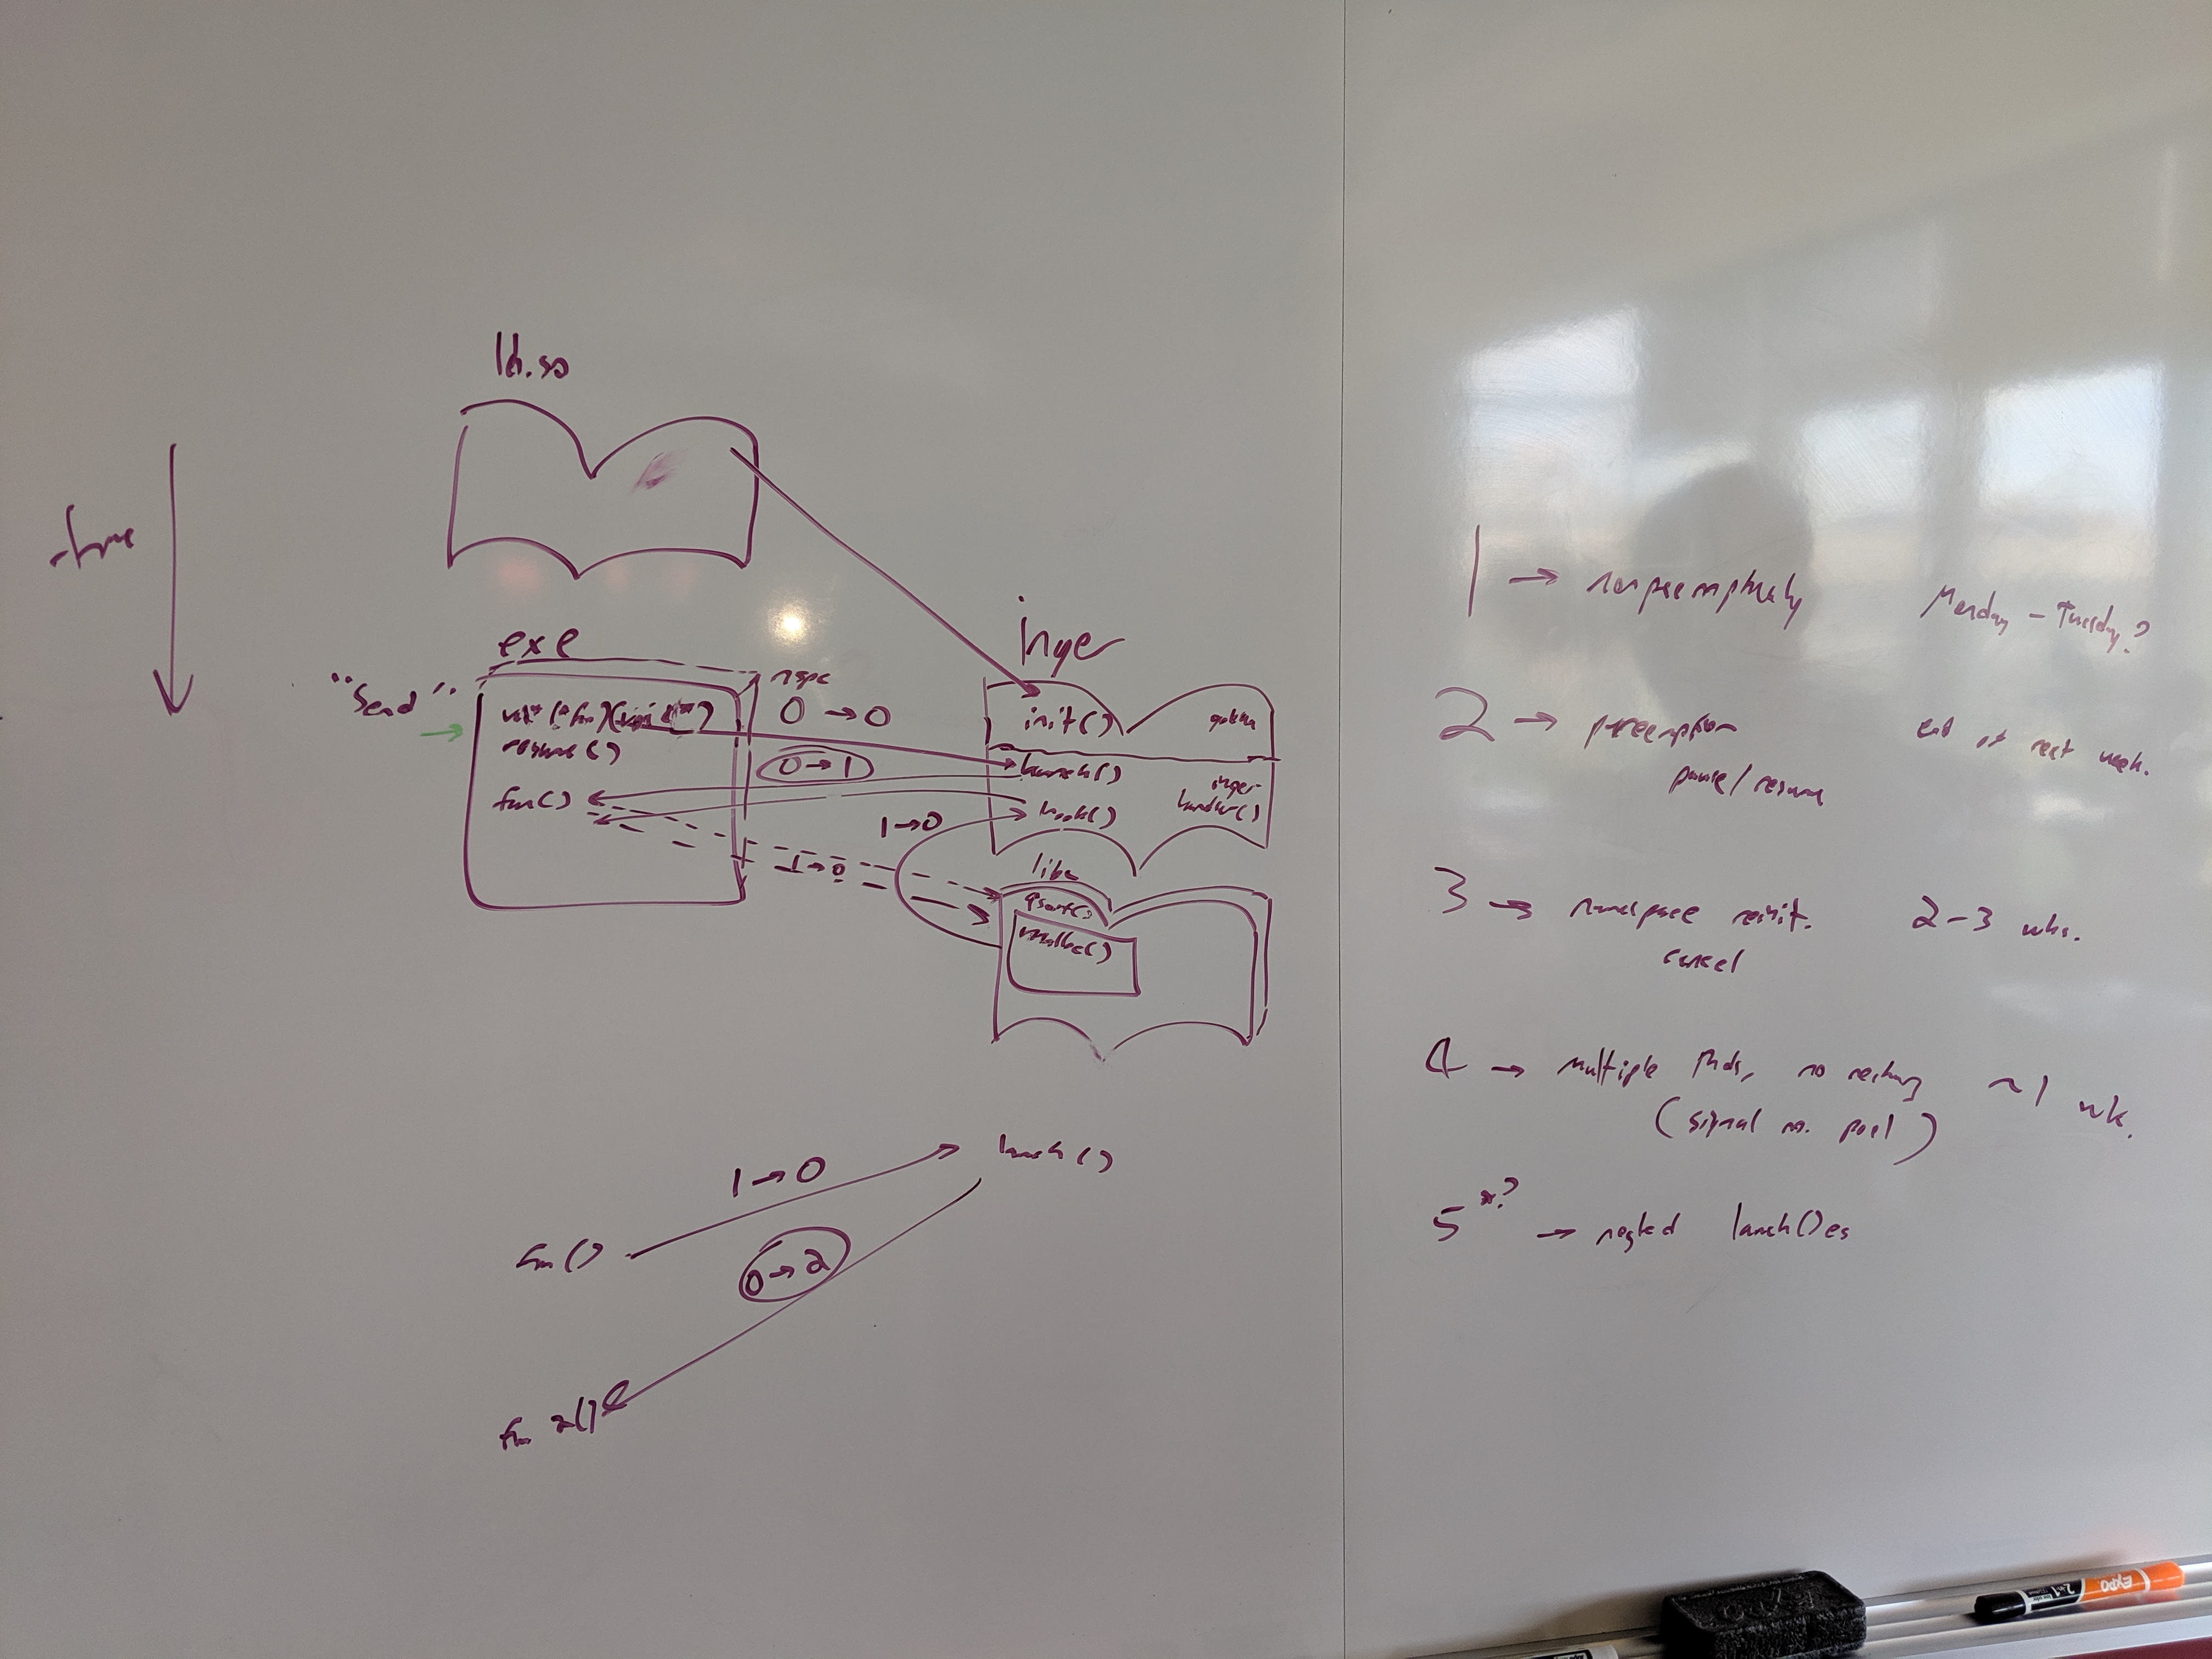
\includegraphics[width=\columnwidth]{figs/calltree}
\caption{How preemptible function dispatch works}
\label{fig:dispatch}
\end{figure}

While the preemptible function is running, the POSIX timer fires periodicially,
causing a signal handler to be invoked each time.  The handler checks whether the
current libset is the main one, indicating that execution is within a shared symbol.
In this case, it blocks the signal and immediately
returns, deferring preemption using libgotcha's callback mechanism in a manner
similar to that discussed in Section~\ref{sec:statefulness}.  Otherwise, if the
preemptible function has exceeded its timeout, the handler swaps the contents of its
third (POSIX context) argument~\cite{sigaction-manpage} with the checkpoint saved by
\texttt{launch()}; this causes the subsequent return from the signal handler to jump
back to \texttt{launch()}, which then returns a \texttt{linger} structure containing
the signal handler's original context.  A subsequent \texttt{resume()} call on this
packaged continuation proceeds in much the same way as \texttt{launch()}, but
resumes the computation on its stack by sending itself a special signal with
\texttt{pthread\_kill()}, then swapping the saved context with the contents of the
handler's third argument.  Figure~\ref{fig:twostacks} shows the two stacks and which
parts of the program execute on each.

\begin{figure}
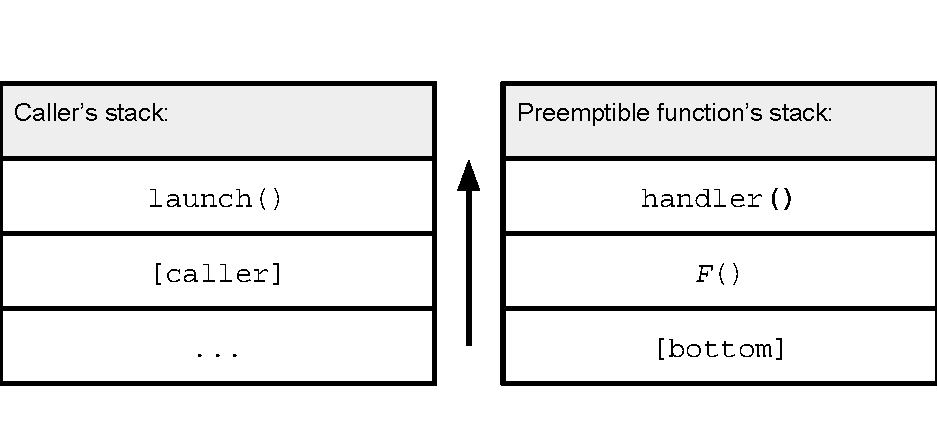
\includegraphics[width=\columnwidth]{figs/twostacks}
\caption{Which code executes on which stack}
\label{fig:twostacks}
\end{figure}

Whenever a preemptible function runs to successful completion, its preemption signal
and libset are reclaimed for reuse by future \texttt{launch()} invocations.  If the
function is canceled rather than being allowed to complete, the libset is assumed to
be in an undefined state and must be reinitialized before reuse.  C client code is
required to explicitly ``deallocate'' continuations upon cancellations, whereas in
Rust the libinger cleanup is performed implicitly by the \texttt{linger} type's
destructor.  While the current implementation performs libset reinitialization
synchronously, given sufficient spare namespaces, this somewhat costly step could be
deferred and handled by a separate reaper thread off the critical path.

The current implementation of libinger does not automatically clean up resources
allocated by preemptible functions that are canceled.  While this is inherently hard
to do in C, it is possible to implement in languages such as Rust that support
destructors.  For instance, the approach proposed by Boucher et
al.~\cite{boucher:atc2018} could be employed to raise a panic (exception) on the
preemptible function's stack, causing the language runtime to unwind each stack frame,
invoking the destructor of each local variable in the process.

While libinger in principle runs on top of an unmodified version of the GNU dynamic
linker, in practice initializing more than one namespace tends to exhaust the
statically-allocated thread-local storage area.  We currently work around this
problem by rebuilding \texttt{ld.so} with the \texttt{TLS\_STATIC\_SURPLUS} macro set
to a larger value.  At the same time, it is possible to raise the default limit
of 16 linker namespaces by increasing the value of \texttt{DL\_NNS}.  With this
change, the only remaining scaling limit is the number of kernel threads running
timed functions, which is limited to the number of signals earmarked for preemption;
however, this number could be increased to over 32 by using realtime
signals~\cite{signal-manpage}, and beyond by rebuilding Linux and glibc with a larger
\texttt{\_NSIG}.

\solb{Mention static linking against libgotcha?}

\solb{Go ``also'' heap-allocates goroutine locals: \url{https://github.com/golang/go/issues/33216}}

\subsection{Case study: Userland threading}
\label{sec:threading}
